\chapter{Proposta Conceitual}

Esta seção apresenta uma proposta de utilização de \textit{templates} hierárquicos para criar e manipular questões de programação. A ideia inclui o emprego de inteligência artificial generativa como ferramenta complementar, responsável por sugerir variações criativas no \textit{template} base, tais como modificações de contexto, acréscimo de novos cenários e introdução de pontos de variação. Além disso, a IA generativa também oferece suporte no fornecimento de \textit{feedback} imediato ao estudante após a submissão da resposta, apontando erros, sugerindo melhorias e apresentando explicações detalhadas sobre o problema e possíveis soluções. 

\subsection{Geral para o Específico}
A geração automática de questões segue um processo hierárquico que se inicia em tópicos mais amplos e evolui até questões específicas. Em primeiro lugar, é definido os tópicos da ementa, que correspondem a áreas ou domínios do conhecimento a serem avaliados (por exemplo, Estruturas de Repetição, Estruturas de Decisão, Matrizes, Funções). Esses tópicos abrangem conteúdos específicos do currículo e orientam a elaboração dos modelos cognitivos. Na etapa seguinte, estes modelos cognitivos são convertidos em \textit{templates}, que servirão de base para a geração das questões. Essa abordagem reflete a metodologia recomendada para a criação de questões baseadas em \textit{templates}. 

\begin{figure}[ht]
	\centering
	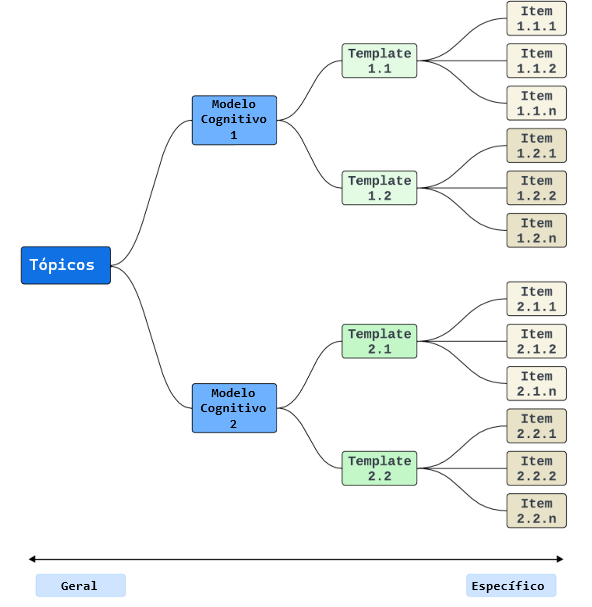
\includegraphics[width=14cm]{./imagens/capitulo5/geral-especifico-com-topicos}
	\caption{Geral para o específico, (adaptado, \cite{hendrickson2010}) }
	\label{fig:geral-to-specif}
\end{figure}


\subsection{Escala de proficiência}

A classificação das questões com base em atributos e características, como o nível de dificuldade, é essencial nas avaliações educacionais. Agrupar questões por níveis de dificuldade (fácil, médio e difícil) possibilita organizar bancos de questões que atendem diferentes perfis de estudantes.  Esse agrupamento é especialmente relevante em contextos que utilizam testes adaptativos , onde o sistema ajusta a dificuldade das questões apresentadas de acordo com o nível de aptidão do aluno. Assim, é possível proporcionar uma experiência de aprendizado personalizada, onde cada questão apresentada se adequa ao desempenho e à evolução do aluno ao longo das avaliações. \textbackslash{}\parencite{pasquali2018}. 


A figura \ref{fig:proficiency-scale}  ilustra um banco de modelos estruturado para oferecer templates compatíveis com diferentes níveis de dificuldade. Esse tipo de organização permite um maior controle sobre a dificuldade das questões geradas.


\begin{figure}[ht]
	\centering
	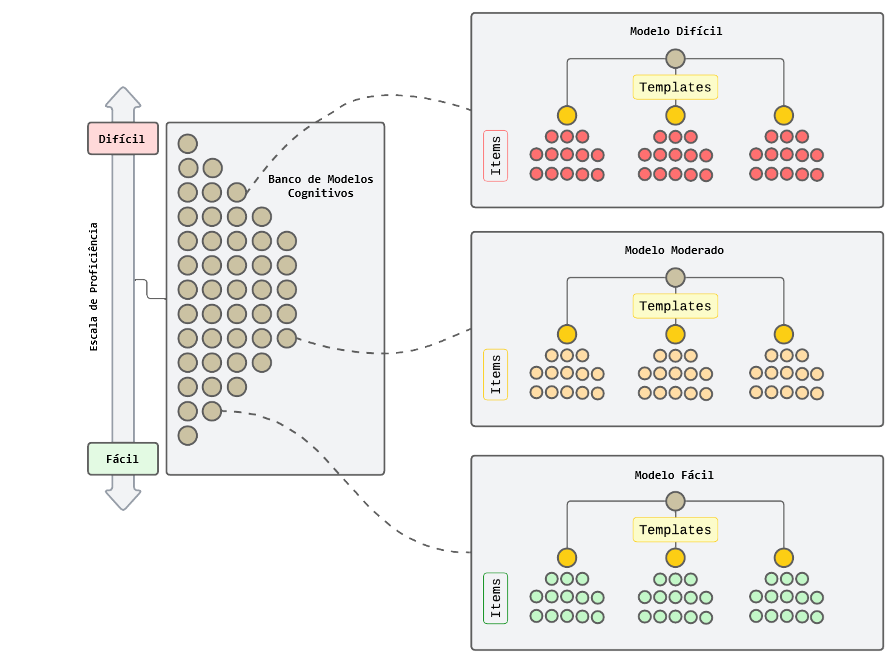
\includegraphics[width=14cm]{./imagens/capitulo5/proficiency-scale-named}
	\caption{Geral para o específico, (adaptado, \cite{hendrickson2010}) }
	\label{fig:proficiency-scale}
\end{figure}

\subsection{Template de Questões com Estrutura Json}

O JSON foi adotado como formato padrão para a construção dos templates de questões devido ao seu alto desempenho, simplicidade e facilidade de uso. Em comparação ao XML, o JSON mostrou-se mais eficiente em diversas métricas, conforme demonstrado no trabalho de \parencite{wang2011}, que indica um ganho de  48,56\% na velocidade de carregamento de 1000 objetos por página comparado com o XML. Esse resultado deve-se, em grande parte, à estrutura mais enxuta do JSON, que demanda menos esforço de interpretação se comparado ao uso extensivo de \textit{tags} no XML.  Além disso, o JSON oferece suporte nativo a tipos de dados como \textit{arrays}, números, \textit{strings} e valores booleanos, o que simplifica o tratamento de estruturas hierárquicas — característica fundamental na representação de templates de questões.


 Outro fator relevante é a compatibilidade natural do JSON com linguagens de programação modernas, como JavaScript, Python e Java, eliminando a necessidade de bibliotecas externas para análise (\textit{parsing}) ou manipulação de dados Por outro lado, o XML frequentemente demanda recursos adicionais para tratamento de \textit{tags} e maior quantidade de código para realizar a análise, acarretando maior esforço de processamento.   A comparação de desempenho realizada por \parencite{goyal2017} reforça essas vantagens ao evidenciar que o JSON, por ser mais leve e simples, apresenta melhor tempo de leitura em aplicações que utilizam pares de chave-valor conforme a figura \ref{fig:json-vs-xml}. Dessa forma, sua utilização torna o desenvolvimento de sistemas mais ágil, eficiente e escalável, justificando a escolha do JSON como formato preferencial para o gerenciamento e representação de templates de questões neste trabalho. 

\begin{figure}[ht]
	\centering
	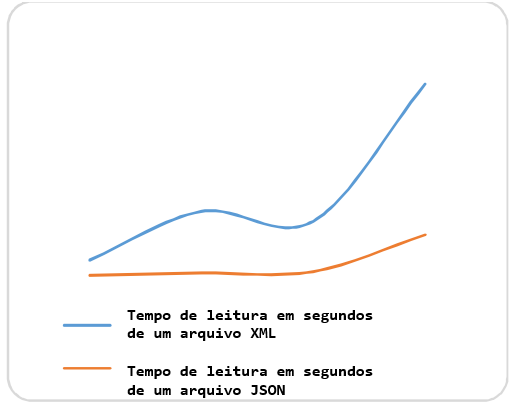
\includegraphics[width=14cm]{./imagens/capitulo5/json-vs-xml}
	\caption{comparação de leitura JSON vs XML, \parencite{goyal2017} }
	\label{fig:json-vs-xml}
\end{figure}


\subsection{Estrutura do Template}

A figura abaixo apresenta uma estrutura hierárquica que representa um template em um arquivo JSON. Podemos ver uma clara definição do texto principal (Stem), assim como o conjunto de variáveis e camadas (layers). Essa organização permite modificar e reutilizar os componentes do template facilmente, conforme necessário. Inicialmente, escrever o modelo de item em um editor de texto é uma prática útil para planejar a estrutura e os elementos das questões. No entanto, a fase seguinte envolve a estruturação desse modelo em formato JSON, o que facilita a manipulação e a geração de questões de forma automatizada. A transição para JSON permite que o template seja facilmente manipulado e gerenciado, promovendo a flexibilidade necessária para ajustar e expandir o banco de questões conforme a necessidade.


\subsection{Mecanismo de Combinação}